\documentclass[10pt,a5paper,twoside,titlepage]{scrartcl}
\usepackage{lmodern}
\usepackage[T1]{fontenc}
\usepackage[utf8]{inputenc}
\usepackage{array}
\usepackage{graphicx}
\usepackage{caption}
\usepackage{subcaption}
\graphicspath{ {sam-screens/}}
\usepackage[ngerman]{babel}
\usepackage{listings}
\usepackage{courier}
\parindent 0pt
\usepackage[pdfborder={0 0 0}]{hyperref}
\usepackage[hyphenbreaks]{breakurl}
\usepackage{floatflt} 
\usepackage[font=small,font=sf,labelfont=sf]{caption}
\usepackage{float}

\title{\LaTeX\ \ -\ Testdokument}
\date{\today}
\author{Valentin Roland}

\lstset{
	tabsize=2,
	breaklines=true,	
	showstringspaces=false,
	basicstyle=\ttfamily,
	breaklines=true
}

\renewcommand\lstlistingname{Quellcode}
\renewcommand{\arraystretch}{1.1} 

\usepackage{fancyhdr}
\pagestyle{fancy}
\renewcommand{\headrulewidth}{0.0pt}
\fancyhead{}
\fancyhead[LE,RO]{\textsf{\rightmark}}
\fancyhead[LO,RE]{\textsf{\leftmark}}
\fancyfoot{}
\fancyfoot[LE,RO]{\thepage}

\usepackage{framed}
\usepackage{xcolor}

% definition of a new float type (refer to the caption package documentation)
\DeclareCaptionType{hwtype}

% definition of a shaded-like environment (see framed.sty)
\newenvironment{myshaded}
  {\def\FrameCommand{\colorbox{shadecolor}}
    \MakeFramed {\advance\hsize-\width \FrameRestore}}
 {\endMakeFramed}

% main environment
% syntax: \begin{myenv}{color}{width}...\end{myenv}
\newenvironment{hinweis}
  {\colorlet{shadecolor}{black!20}%
      \begin{myshaded}
      \begin{minipage}{\linewidth}
      %\parindent 20pt
	  \hangindent 20pt  
      \textbf{Hinweis:}\\
      }
  {\end{minipage}\end{myshaded}}
  
\newenvironment{warnung}
  {\colorlet{shadecolor}{yellow!20}%
      \begin{myshaded}
      \begin{minipage}{\linewidth}
      %\parindent 20pt
	  \hangindent 20pt  
      \textbf{Warnung:}\\
      }
  {\end{minipage}\end{myshaded}}

\captionsetup[subfigure]{labelformat=empty}
\def\pkname{SimpleAnalyzer}

\title{\pkname}
\author{Handbuch}
\date{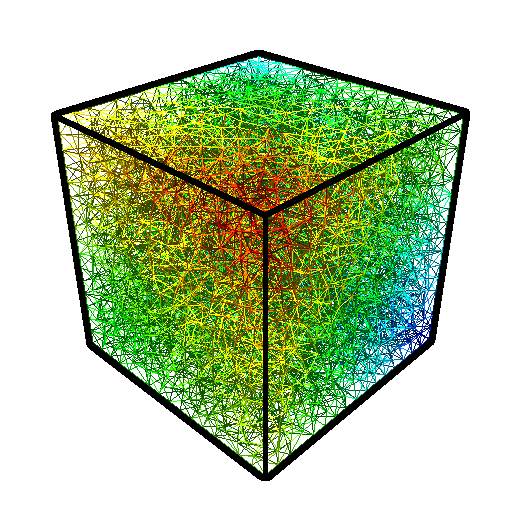
\includegraphics[width=.8\linewidth]{doc_icon.png}}

\begin{document}
	\begin{titlepage}
		\Huge{\textbf{\pkname}}\\
		\Huge{Handbuch}
		\vfill
   		\begin{center}
   		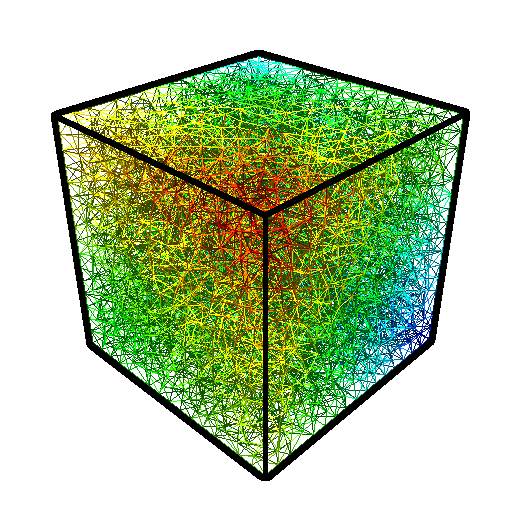
\includegraphics[width=\linewidth]{doc_icon.png}
   		\end{center}
	\end{titlepage} 
	
	\tableofcontents
	\newpage
	\section{Einführung}
	Das \pkname -Softwarepaket enthält Programme zur Auswertung physikalischer Versuche für debianbasierte Betriebssysteme. 
	Mithilfe der enthaltenen Software sind Sie im Stande, Temperaturmessdaten aus einer .csv-Datei oder Messwerte des ODiSI-Instruments von Luna in ein einheitliches Format umzuwandeln und zusammenzuführen.\\
	Über eine grafische Oberfläche ist es möglich, mithilfe der so aufbereiteten Daten Auswertungen wie eine Temperaturverteilung über ein dreidimensionales Modell oder das Bestimmen des Wärmegehalts vorzunehmen und den Versuch zu visualisieren.\\
	Zur weiteren Nutzung der Ergebnisse können diese, beispielsweise als VTK-Datei oder PNG-Grafik, exportiert werden.
	\newpage
	\section{Installation}
	\subsection{Download}
	Falls Sie keine Kopie der Software auf einem Datenträger besitzen oder eine neue Version der Software beziehen möchten,
	müssen Sie die Software zuerst herunterladen.
	\subsubsection{Download des Debian-Packets}
	\label{subsec:deb_download}
	Wenn sie nur die Programme benötigen, reicht es aus das Debian-Paket für Ihr System, sofern verfügbar, herunterzuladen. Navigieren Sie dazu mit ihrem Browser zur Adresse \url{https://github.com/vroland/SimpleAnalyzer/tree/master/deb-bin} und laden sie die Datei
	\begin{lstlisting}
	simpleanalyzer_<version>_<architektur>.deb
	\end{lstlisting}
	herunter. Dabei ist \emph{<version>} die gewünschte Version und \emph{<architektur>} die gewünschte Systemarchitektur.
	Für \emph{<version>} sollten Sie stets die neueste, also die höchste verfügbare Nummer auswählen.
	Wenn Sie nicht wissen, welchen Wert sie für \emph{<architektur>} auswählen müssen, führen sie den Befehl 
	\begin{lstlisting}
	dpkg --print-architecture	
	\end{lstlisting}
	in einem Terminal aus. Bei Fragen zur Nutzung des Terminals, ziehen Sie die Hilfe ihrer Distribution zu Rate.
\begin{hinweis}
	 Eine Einführung in die Terminalnutzung unter Ubuntu finden sie unter  \url{http://wiki.ubuntuusers.de/Terminal}.
	\end{hinweis}
	 Der zurückgegebene Wert ist ihr Wert für \emph{<architektur>}.\\
	Falls kein Paket für ihre Architektur vorhanden ist, fahren Sie mit
	\ref{subsec:download_code} fort.
	\subsubsection{Download des Quellcodes}
	\label{subsec:download_code}
	Benötigen Sie auch Beispieldateien, Quellcode oder existiert kein fertiges Paket für ihr System, müssen Sie alle Dateien aus dem \pkname-Repository herunterladen. Folgen Sie dazu dem Link	\url{https://github.com/vroland/SimpleAnalyzer/archive/master.zip}
	und laden Sie das die Zip-Datei herunter. Extrahieren Sie die Datei anschließend mithilfe der Archivverwaltungssoftware ihres Systems in ein Verzeichnis ihrer Wahl. Wenn Sie später auf Beispiele oder Quelltext zurückgreifen wollen, bietet sich hierfür Ihr HOME-Verzeichnis an. Informationen zum Entpacken von Archiven für die meisten debianbasierten Distributione finden Sie unter \url{http://wiki.ubuntuusers.de/Archivmanager}.\\
	Wenn sie mit der Nutzung des Programms \emph{git} vertraut sind, können Sie alternativ auch folgende clone-URL verwenden:\\
	
	\url{https://github.com/vroland/SimpleAnalyzer.git}
	\subsection{Installation Im Dateisystem}
	\label{subsec:install}
	Zur Installation des \pkname -Programmpakets haben Sie mehrere Möglichkeiten. 
	\begin{hinweis}
	Um die Installation durchführen zu können benötigen Sie Administrator(Superuser)-Rechte (zu erkennen an der Verwendung des \emph{sudo}-Schlüsselworts). Wenn Sie das während der Installation abgefragte Passwort nicht kennen, wenden Sie sich an Ihren Systemadministrator. 
	\end{hinweis}
	\subsubsection{Installation des Debian-Pakets}
	\label{subsec:install_from_package}
	\begin{warnung}
	Wenn Sie die Software bereits aus dem Quellcode installiert haben, deinstallieren Sie die Software vorher, wie in \ref{subsec:uninstall_code} beschrieben!
	\end{warnung}
	Die Verwendung eines Debian-Pakets ist die einfachste und schnellste Möglichkeit, die Programme auf dem Computer zu installieren. Die Paket-Datei erkennen sie am Dateinamen:
	\begin{lstlisting} 
	simpleanalyzer_<version>_<architektur>.deb
	\end{lstlisting}
	\emph{<version>} entspricht der Version des Programms und \emph{<architektur>} der Systemarchitektur, für die das Paket erstellt ist. Sie sollte mit ihrem System übereinstimmen. Wie sie ihre Systemarchitektur ermitteln, können sie in \ref{subsec:deb_download} nachlesen.
	Sollten Sie keine solche Datei finden können, müssen Sie diese erst herunterladen, wie in \ref{subsec:deb_download} beschrieben. Falls kein Paket für ihr System zu Verfügung steht, fahren Sie stattdessen mit \ref{subsec:install_from_source} fort.\\
	Öffnen Sie ein Terminal und navigieren sie zu dem Verzeichnis, in dem die Paketdatei liegt. Führen sie nun den Befehl
	\begin{lstlisting}
	sudo dpkg -i simpleanalyzer_<version>_<architektur>.deb
	\end{lstlisting}
	aus und geben sie gegebenenfalls erfragte Informationen ein.
	Nun sind die alle benötigten Programme installiert.
	\begin{hinweis}
	Wenn sich die Paket-Datei auf einem NTFS- oder FAT-formatierten Datenträger befindet, wird auf manchen Systemen eine Warnung ausgegeben, nach der das Paket von  	\emph{schlechter Qualität} sei. Um dies zu vermeiden, sollte sich die Datei nicht auf einem solchen Datenträger befinden.
	\end{hinweis}	
	Unter manchen Distributionen genügt es, wenn sie einen Doppelklick auf das Paket durchführen und auf \textbf{[Installieren]}-Button im sich öffnenden Fenster zu klicken.
	
	\begin{figure}
	\centering	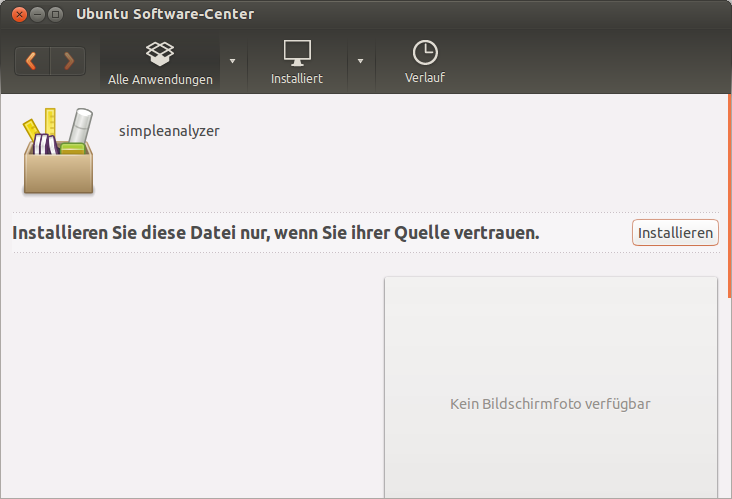
\includegraphics[clip=true,trim=0 5cm 0 0,scale=.3]{Ubuntu_Software_Center_002.png}
	\caption{Installation im Ubuntu Software Center}
	\end{figure}
		
	\subsubsection{Installation aus dem Quellcode}
	\label{subsec:install_from_source}
	\begin{warnung}
	Wenn Sie bereits ein Debian-Paket der Software installiert haben, deinstallieren Sie dieses vorher, wie in \ref{subsec:uninstall_debian} beschrieben!
	\end{warnung}
	Nachdem Sie dem Quellcode wie in \ref{subsec:download_code} beschrieben heruntergeladen und entpackt haben, öffnen Sie ein Terminal und navigieren Sie in das entpackte Verzeichnis. Wenn Sie hier den Befehl
	\begin{lstlisting}
	ls
	\end{lstlisting}
	ausführen, sollte unter anderem eine Datei Namens \grqq makefile\grqq\space aufgelistet werden. Anderenfalls überprüfen Sie, ob Sie die heruntergeladene Datei vollständig entpackt haben und Sie sich mit dem Terminal in diesem Verzeichnis befinden.
	Um die Programme nun aus dem Quelltext zu erstellen, sind weitere Pakete nötig. Für die meisten Distributionen sind diese Pakete in den offiziellen Softwarequellen enthalten, können also über den Paketmanager ihrer Distribution installiert werden. Hier die entsprechenden Befehle am Beispiel von Ubuntu:
	\begin{lstlisting}
	sudo apt-get update
	sudo apt-get install build-essential wx-common wx2.8-headers libwxgtk2.8-dev libwxbase2.8-dev libwxbase2.8-0 libwxgtk2.8-0
	\end{lstlisting}
	Falls ihr System einen anderen Paketmanager verwendet, entnehmen Sie Anweisungen zu dessen Verwendung aus der Hilfe ihrer Distribution.\\
	Nun können Sie die Programme durch Ausführen des Befehls
	\begin{lstlisting}
	make
	\end{lstlisting}
	Erstellen. Um die Programme nun mit allen benötigten Dateien zu Installieren, führen Sie den Befehl
	\begin{lstlisting}
	sudo make install
	\end{lstlisting}
	\begin{warnung}
	Wenn Sie ein eigenes Installationspräfix gewählt haben (hier nicht beschrieben), beachten Sie, dass die von den Programmen benötigten Daten nur unter folgenden Pfaden gesucht werden:\\
	/usr/local/share/simpleanalyzer\\
	/usr/share/simpleanalyzer\\
	Verzeichnis der ausführbaren Datei
	\end{warnung}
	aus. Die Installation ist nun abgeschlossen.
	\begin{hinweis}
	Die Pakete \emph{build-essential, wx2.8-headers, libwxgtk2.8-dev} und \emph{libwxbase2.8-dev} werden nicht zum Betrieb des Programms benötigt, könnten also später wieder entfernt werden. Die übrigen hingegen sind für das Funktionieren der Programme essentiell.
	\end{hinweis}
	\subsection{Deinstallation}
	Wenn Sie das \pkname -Programmpaket wieder deinstallieren möchten hängt ihr Vorgehen von der verwendeten Installationsmethode ab.
	\begin{warnung}
	Wenn Sie die Software als Debian-Paket installiert haben (s. \ref{subsec:install_from_package}), folgen Sie zum deinstallieren dem Abschnitt \ref{subsec:uninstall_debian}!\\
	Haben Sie die Software aus dem Quellcode installiert (s. \ref{subsec:install_from_source}), folgen Sie zum Deinstallieren dem Abschnitt \ref{subsec:uninstall_code}!
	\end{warnung}
	\subsubsection{Deinstallation des Debian-Pakets}
	\label{subsec:uninstall_debian}
	Um das Debian-Paket zu deinstallieren, öffnen Sie ein Terminal und führen Sie den Befehl
	\begin{lstlisting}
	sudo dpkg -r simpleanalyzer
	\end{lstlisting}
	aus. 
	\subsubsection{Deinstallation durch den Quellcode}
	\label{subsec:uninstall_code}
	Wenn sie die Installation aus dem Quellcode rückgängig machen wollen, öffnen Sie ein Terminal und navigieren Sie wie bereits bei der in \ref{subsec:install_from_source} beschriebenen Installation in das Verzeichnis, das den Quellcode enthält.
	Führen Sie nun
	\begin{lstlisting}
	sudo make uninstall
	\end{lstlisting}
	aus, um die Software zu deinstallieren.
	\newpage
	\section{Verwendung}
	Das \pkname -Programmpaket enthält vier Einzelprogramme. Hier sehen Sie eine Übersicht über die Programme und deren Funktion:\\
	
	\begin{tabular}{p{.31\linewidth}|p{.58\linewidth}}
	\textsc{Programm} & \textsc{Funktion}\\
	\hline
	csvtosd & Wandelt Sensordaten von Character-separated values (.csv)-Dateien zu timed sensor data (.tsd)-Dateien um.\\
	&\\
	odisitosd & Wandelt Messwertdateien des ODiSI-Instruments in .tsd-Dateien um.\\
	&\\
	mergetsd & Fügt zwei .tsd-Dateien zusammen.\\
	&\\
	simpleanalyzer-gui & Berechnet mithilfe eines 3D-Modells des Versuchs eine Temperaturverteilung, visualisiert diese und ermittelt für die Auswertung des Versuchs wichtige Werte.
	\end{tabular}
	\begin{hinweis}
	Die Anwendung der Programme an einem Beispiel finden sie unter \ref{sec:example}.
	\end{hinweis}
	\newpage
	
	
	\subsection{Umwandeln von .csv-Dateien}
	\label{subsec:csvtosd}
	Um Messwerte, die als .csv-Dateien vorliegen in das von \emph{sim"-ple"-ana"-ly"-zer-gui} genutzte .tsd-Format (timed sensor data) umzuwandeln, verwenden Sie das Programm \emph{csvtosd}. Das Programm wird über das Terminal ausgeführt. Dabei werden Einstellungen zur Umwandlung nach folgendem Muster festgelegt:
	\begin{lstlisting}
	csvtosd <argument1> <wert1> <argument2> <wert2> ...
	\end{lstlisting}
	Mögliche Argumente (teilweise mit alternativer Kurzform):\\
	
	\begin{tabular}{p{.2\textwidth}c|p{.6\textwidth}}
	-in & -i & \textbf{[benötigt]} Pfad zur umzuwandelnden .csv-Datei\\
	-out & -o & \textbf{[benötigt]} Pfad zur Ausgabedatei\\
	-sensor-def & -s & \textbf{[benötigt]} Pfad zur Sensordefinitions-Datei (s. \ref{subsec:sdef_csvtosd})\\
	-step-time & & [optional] nur jeden n-ten Datensatz verwenden\\
	-min-time & & [optional] erst ab diesem Zeitpunkt umwandeln\\
	-max-time & & [optional] nur bis zu diesem Zeitpunkt umwandeln\\
	-help & -h & [optional] Einen Hilfetext ausgeben \\
	&&\emph{benötigt keinen Wert}
	\end{tabular}
	\begin{hinweis}{}
	Wenn sie einen Pfad angeben wollen, der Leerzeichen enthält, müssen Sie ihn in Anführungszeichen setzen.\\
	z.B. docs/ordner 1/i.csv $\rightarrow$ \dq docs/ordner 1/i.csv\dq
	\end{hinweis}
	
	\begin{warnung}
	Alle verwendeten Dateien sollten, um Fehlfunktionen auszuschließen, ASCII-codiert und mit Linux-zeilenenden versehen sein. Um eine Textdatei entsprechend umzuwandeln, verwenden Sie den Befehl:
	\begin{lstlisting}
	dos2unix <Datei>
	\end{lstlisting}
	\end{warnung}
	\subsubsection{Die .csv-Datei}
	Damit eine .csv-Datei vom Programm gelesen werden kann, muss sie folgende Kriterien erfüllen:
	\begin{itemize}
	\item Die Datei muss eine Zeile enthalten, in der die Namen der Spalten stehen (Kopfzeile). Die Spaltennamen für die Sensordaten müssen denen in der Sensordefinitionsdatei entsprechen. Weiterhin muss eine Spalte die Zeit für die Datensätze enthalten.
	\begin{warnung}
	Die Werte der Zeitspalte werden als Ganzzahl interpretiert. Die Einheit sollte also entsprechend genau gewählt werden, bspw. $Sekunden$.
	\end{warnung}
	\item Es können beliebig viele zusätzliche Spalten vor und nach den Sensordatenspalten stehen, wie z.B. Namen für die Datensätze. Sie müssen jedoch sicherstellen, dass ihre Konfigurationsdatei (s. \ref{subsec:conf_csvtosd}) die dementsprechenden Einstellungen enthält.
	\item Unter der Kopfzeile folgen die Datensätze zeilenweise mit den jeweiligen Daten für alle Spalten.
	\item Während sich vor der Kopfzeile noch zusätzliche Zeilen befinden können (s. \ref{subsec:conf_csvtosd}), darf die Datei nach der letzten Sensordatenzeile keinen Eintrag mehr enthalten.
	\end{itemize}
	\begin{hinweis}
	Wenn ihre Datei diesen Anforderungen nicht entspricht und die  Konfigurationsdatei (s. \ref{subsec:conf_csvtosd}) keine entsprechenden Optionen enthält, können Sie einen Texteditor oder ein Tabellenverarbeitungsprogramm nutzen, um eine kompatible Datei zu erstellen.
	\end{hinweis}
	\subsubsection{Die Sensordefinitionsdatei}
	\label{subsec:sdef_csvtosd}
	Neben der Eingabedatei müssen Sie auch eine Sensordefinitionsdatei angeben, in der Informationen zu der in der Eingabedatei genutzten Sensoren abgelegt sind. Die Sensordefinitionsdatei ist eine Textdatei und ist nach folgendem Schema aufgebaut:\\
	\begin{lstlisting}
	name1 x1 y1 z1
	name2 x1 y1 z1
	...
	\end{lstlisting}
	\begin{hinweis}
	Sie können Zeilen als Kommentar markieren, indem Sie diese Zeile mit \emph{\#} beginnen. Die betreffende Zeile wird dadurch nicht ausgewertet.
	\end{hinweis}
	Nach dem Sensornamen folgt die Position des Sensors in kartesischen Koordinaten, jeweils durch Leerzeichen getrennt.
	\textbf{Die Sensornamen müssen dabei den entsprechenden Spaltennamen in der umzuwandelnden .csv-Datei entsprechen!}
	\begin{hinweis}
	Wenn die Sensornamen Leerzeichen enthalten, müssen Sie diese in Anführungszeichen setzen.\\
	z.B. Sensor 1 1.5 0.5 1.0 $\rightarrow$ \dq Sensor 1\dq \space 1.5 0.5 1.0
	\end{hinweis}
	\subsubsection{Die Konfigurationsdatei}
	\label{subsec:conf_csvtosd}
	Zusätzlich sind allgemeine Einstellungen zum Programm in einer Konfigurationsdatei gespeichert. Sie befindet sich, sofern Sie die in \ref{subsec:install} beschriebenen Schritte befolgt haben, in folgendem Verzeichnis:
	\begin{lstlisting}
	/etc/simpleanalyzer/csvtosd.conf
	\end{lstlisting}
	Die Konfigurationsdatei ist eine Textdatei, wobei der Wert für jede Einstellung auf einer bestimmten Zeile steht. Sie hat folgenden Aufbau:\\
	
	\newcounter{rownum}
	\setcounter{rownum}{0}
	\textsc{Zeile} / \textsc{Standardwert} / \textsc{Beschreibung}\\
	
	\begin{tabular}{p{.03\textwidth}|p{.02\textwidth}|p{.8\textwidth}}
	\addtocounter{rownum}{1}\arabic{rownum} & 4 & Index der ersten Spalte in der .csv-Datei, die Sensordaten enthält\\
	\addtocounter{rownum}{1}\arabic{rownum} & ; & Zeichen zur Spaltenabtrennung\\
	\addtocounter{rownum}{1}\arabic{rownum} & 1 & Komma als Dezimaltrennzeichen zulassen\\
	\addtocounter{rownum}{1}\arabic{rownum} & 2 & Index der Zeitspalte (als Zeitstempel)\\
	\addtocounter{rownum}{1}\arabic{rownum} & 1 & Index der als Datensatzname verwendeten Spalte\\
	\end{tabular}
	\begin{hinweis}
	Indices werden Null-basiert angegeben. \\
	z.B. Die \emph{3.} Spalte hat den Index \emph{2}.
	\end{hinweis}
	\newpage
	\subsection{Umwandeln von ODiSI-Dateien}
	\label{subsec:odisitosd}
	Um Messwerte aus einer ODiSI-Dateien vorliegen in das von \emph{simple\-analyzer-gui} genutzte .tsd-Format (timed sensor data-Format) umzuwandeln, verwenden Sie das Programm \emph{odisitosd}.
	\emph{Zusätzlich können Ausreißer in den Messdaten korrigiert werden.}
	Der Aufruf erfolgt wie bei csvtosd (s. \ref{subsec:csvtosd}):
	\begin{lstlisting}
	odisitosd <argument1> <wert1> <argument2> <wert2> ...
	\end{lstlisting}
	Mögliche Argumente (teilweise mit alternativer Kurzform):\\
	
	\begin{tabular}{p{.2\textwidth}c|p{.6\textwidth}}
	-in & -i & \textbf{[benötigt]} Pfad zur umzuwandelnden Datei\\
	-out & -o & \textbf{[benötigt]} Pfad zur Ausgabedatei\\
	-sensor-def & -s & \textbf{[benötigt]} Pfad zur Sensordefinitions-Datei (s. \ref{subsec:sdef_odisitosd})\\
	-log & -l & [optional] Pfad zur Log-Datei\\
	-height & & [optional][Standardwert in der Konfigurationsdatei festgelegt]\\&& Die Höhe der Faserebene\\
	-step-time & & [optional] nur jeden n-ten Datensatz verwenden\\
	-step-time & & [optional] nur jeden n-ten Messpunkt auf der Faser verwenden\\
	-min-time & & [optional] erst ab diesem Zeitpunkt umwandeln\\
	-max-time & & [optional] nur bis zu diesem Zeitpunkt umwandeln\\
	-help & -h & [optional] Einen Hilfetext ausgeben \\
	&&\emph{benötigt keinen Wert}
	\end{tabular}\\
	
	Wenn Sie für die Log-Datei einen Pfad angeben, wird eine Log-Datei erstellt. Wenn ein Wert durch die Messwertkorrektur geändert wird oder die Berechnung eines neuen Wertes fehlschlägt, wird eine Bemerkung in diese Datei geschrieben. Diese Bemerkung enthält den alten Wert, die Position in der Datei und ggf. den neuen Wert.
	\begin{hinweis}
	Wenn sie einen Pfad angeben wollen, der Leerzeichen enthält, müssen Sie ihn in Anführungszeichen setzen.\\
	z.B. docs/ordner 1/i.txt $\rightarrow$ \dq docs/ordner 1/i.txt\dq
	\end{hinweis}
	
	\begin{warnung}
	Alle verwendeten Dateien sollten, um Fehlfunktionen auszuschließen, ASCII-codiert und mit Linux-zeilenenden versehen sein. Um eine Textdatei entsprechend umzuwandeln, verwenden Sie den Befehl:
	\begin{lstlisting}
	dos2unix <Datei>
	\end{lstlisting}
	\end{warnung}
	\newpage
	\subsubsection{Die Eingabedatei}
	Damit eine Eingabedatei mit ODiSI-Messwerten vom Programm gelesen werden kann, muss sie folgende Kriterien erfüllen:
	\begin{itemize}
	\item Die Spalten der Datei sind durch ein \textbf{Tabualtorzeichen (als \textbackslash t umschreibbar)} getrennt.
	\item Die Datei muss eine Zeile enthalten, in der die Namen der Spalten stehen (Kopfzeile). Die erste Spalte muss die Zeit für die Sensordaten enthalten, anschließend folgen die Spalten mit den Sensordaten. Die Namen der Sensordatenspalten sind ihre Positionen auf der Faser in der selben Einheit wie in der Sensordefinitionsdatei. Es dürfen keine weiteren Spalten folgen.
	\begin{warnung}
	Die Werte der Zeitspalte werden als Ganzzahl interpretiert. Die Einheit sollte also entsprechend genau gewählt werden, bspw. $Sekunden$.
	\end{warnung}
	\item Unter der Kopfzeile folgen die Datensätze zeilenweise mit Zeit und Temperaturdifferenzen der einzelnen Messpunkte zum Grundwert (s. \ref{subsec:conf_odisitosd}).
	\item Während sich vor der Kopfzeile noch zusätzliche Zeilen befinden können (s. \ref{subsec:conf_odisitosd}), darf die Datei nach der letzten Sensordatenzeile keinen Eintrag mehr enthalten.
	\end{itemize}
	\begin{hinweis}
	Wenn ihre Datei diesen Anforderungen nicht entspricht und die  Konfigurationsdatei (s. \ref{subsec:conf_odisitosd}) keine entsprechenden Optionen enthält, können Sie einen Texteditor oder ein Tabellenverarbeitungsprogramm nutzen, um eine kompatible Datei zu erstellen.
	\end{hinweis}
	
	\subsubsection{Fehlerkorrektur}
	Das odisitosd-Werkzeug ist in der Lage, Ausreißer in den Messwerten zu erkennen und zu bereinigen.
	Dazu wird für jeden Messwert geprüft, ob die Temperaturdifferenz zum vorherigen Wert an dieser Stelle eine bestimmte Schwelle überschreitet. Wenn dies der Fall ist, sucht das Programm unter den nächsten Messwerten einen Wert, für den die Temperaturdifferenz nicht größer als der \textbf{Schwellenwert mal maximale Differenz} ist.\\
	Wird ein solcher Wert gefunden, werden die dazwischen liegenden Ausreißer-werte durch \textbf{linear zwischen den beiden gültigen Punkten interpoliert}.
	Die maximale Temperaturdifferenz und die maximale Suchweite können in der Konfigurationsdatei angegeben werden. (s. \ref{subsec:conf_odisitosd})
	\subsubsection{Die Sensordefinitionsdatei}
	\label{subsec:sdef_odisitosd}
	Neben der Eingabedatei müssen Sie auch hier eine Sensordefinitionsdatei angeben, in der Informationen zum Faserverlauf abgelegt sind. Die Sensordefinitionsdatei ist eine Textdatei und ist nach folgendem Schema aufgebaut:\\
	\begin{lstlisting}
	#Kommentar
	i l1 x1
	o l2 x2
	i l3 x3
	o l4 x4
	...
	d +-+-
	\end{lstlisting}
	\begin{warnung}
	Die Ein- und Ausgänge der Faser müssen nach aufsteigender Position auf der Faser (Länge) sortiert werden. Der Faserausgang besitzt dabei immer eine größere Länge als der Eingang.
	\end{warnung}
	Es werden in zwei aufeinander folgenden Zeilen stets Ein- und Ausgangspunkt der Faser beschrieben (durch \emph{i} bzw \emph{o} markiert). $l_1...l_n$ ist dabei die Position auf der Faser, also die Länge des Verlaufs der Faser bis zu diesem Punkt. $x_1...x_n$ ist die Position auf der X-Achse. Das für den Versuch verwendete Koordinatensystem muss ggf. entsprechend des Faserverlaufs festgelegt werden.	\\
	Optional können Sie für alle Faserdurchläufe durch das Material, die jeweils durch Ein- und Ausgangspunkt eingegrenzt sind, die Richtung des Faserverlaufes fest legen. Fügen Sie dazu eine Zeile hinzu, die mit \emph{d} eingeleitet wird. Nach einem Leerzeichen folgt für jeden Faserdurchlauf dessen (Fädel-)Richtung als positiv (+) oder negativ (-). Wird die Faser also bspw. abwechselnd von vorn und  hinten durch das Versuchsobjekt gefädelt, ergibt sich Abwechseln der Faserrichtung (+-+-).
	\subsubsection{Die Konfigurationsdatei}
	\label{subsec:conf_odisitosd}
	Zusätzlich sind allgemeine Einstellungen zum Programm in einer Konfigurationsdatei gespeichert. Sie befindet sich, sofern Sie die in \ref{subsec:install} beschriebenen Schritte befolgt haben, in folgendem Verzeichnis:
	\begin{lstlisting}
	/etc/simpleanalyzer/odisitosd.conf
	\end{lstlisting}
	Die Konfigurationsdatei ist eine Textdatei, wobei der Wert für jede Einstellung auf einer bestimmten Zeile steht. Sie hat folgenden Aufbau:\\
	
	\setcounter{rownum}{0}
	\textsc{Zeile} / \textsc{Standardwert} / \textsc{Beschreibung}\\
	
	\begin{tabular}{p{.03\textwidth}|p{.05\textwidth}|p{.76\textwidth}}
	\addtocounter{rownum}{1}\arabic{rownum} & 4 & Index der ersten Zeile in der ODiSI-Datei, die Sensordaten enthält\\
	\addtocounter{rownum}{1}\arabic{rownum} & 1 & Komma als Dezimaltrennzeichen zulassen\\
	\addtocounter{rownum}{1}\arabic{rownum} & 5 & Maximal zulässige Differenz zum Vorgängerwert für einen gültigen Messwert\\
	\addtocounter{rownum}{1}\arabic{rownum} & 10 & Maximale Schrittanzahl zum finden eines gültigen Messwertes\\
	\addtocounter{rownum}{1}\arabic{rownum} & 8 & Anzahl der Leerzeichen für TAB (Für die Positionsangabe in der Log-Datei)\\
	\addtocounter{rownum}{1}\arabic{rownum} & 20 & Temperatur zu Beginn des Versuches (Die ODiSI-Daten sind Differenzen zu dieser Anfangstemperatur)\\
	\addtocounter{rownum}{1}\arabic{rownum} & 1 & Position auf der X-Achse spiegeln\\
	\addtocounter{rownum}{1}\arabic{rownum} & .06 & Standardwert für die Höhe der Faserebene\\
	\addtocounter{rownum}{1}\arabic{rownum} & .5 & Position auf der X-Achse um diesen Wert verschieben\\
	\end{tabular}
	\begin{hinweis}
	Indices werden Null-basiert angegeben. \\
	z.B. Die \emph{3.} Spalte hat den Index \emph{2}.
	\end{hinweis}
	\subsection{Zusammenfügen von .tsd-Dateien}
	\label{subsec:mergetsd}
	Um die nun im .tsd-Format vorliegenden Messdaten zusammenzuführen, verwenden Sie das Werkzeug \emph{mergetsd}. Dabei fügt das Programm Datensätze aus beiden Eingabedateien zusammen, deren Zeitstempel annähernd gleich sind.\\
	Der Aufruf erfolgt nach dem bereits in \ref{subsec:csvtosd} gezeigten Muster:
	\begin{lstlisting}
	mergetsd <argument1> <wert1> <argument2> <wert2> ...
	\end{lstlisting}
	Mögliche Argumente (teilweise mit alternativer Kurzform):\\
	
	\begin{tabular}{p{.13\textwidth}c|p{.68\textwidth}}
	-in1 & -i1 & \textbf{[benötigt]} Pfad zur ersten .tsd-Datei. Aus dieser Datei werden die Namen für die zusammengeführten Datensätze entnommen.\\
	-in2 & -i2 & \textbf{[benötigt]} Pfad zur zweiten .tsd-Datei.\\
	-out & -o & \textbf{[benötigt]} Pfad zur Ausgabedatei\\
	-height & & [optional][Standardwert in der Konfigurationsdatei festgelegt]\\&& Die Höhe der Faserebene\\
	-max-dt & & [optional] Maximale Zeitdifferenz zwischen den Zeitstempeln (Standardwert: 3)\\
	-auto-offset & & [optional] Zu den Zeitstempeln der zweiten Datei die Differenz der jeweils ersten Datensätze addieren (true/false oder 1/0, Standardwert: true)\\
	-offset & & [optional] Ein zusätzlicher Versatz, der zu den Zeitstempeln der zweiten Datei addiert wird\\
	-help & -h & [optional] Einen Hilfetext ausgeben \\
	&&\emph{benötigt keinen Wert}
	\end{tabular}\\
	\newpage
	\subsection{Erstellung des 3D-Modells}
	\label{subsec:usage_model}
	Zur Auswertung des Versuchs wird auch ein Modell des zu untersuchenden Objekts benötigt. Um dieses zu erstellen können Sie ein beliebiges Werkzeug verwenden, wenn dieses in der Lage ist, Modelle im \textbf{Wavefront (.obj)-Format} zu erstellen. Zur .obj-Datei muss eine Materialbibliothek-Datei (.mtl) mit Informationen über die verwendeten Materialien vorliegen.\\
	\emph{Objekte mit mehreren Materialien müssen durch mehrere geschlossene Teilobjekte mit jeweils eigenem Material erstellt werden.}
	\begin{hinweis}
	Informationen zum Aufbau dieser Dateien finden Sie unter \url{http://en.wikipedia.org/wiki/Wavefront_.obj_file}.
	\end{hinweis}
	\begin{hinweis}
	Über das Attribut \emph{density} in der .mtl-Datei können Sie die  Dichte eines Materials in $\frac{kg}{m^3}$ und mit \emph{spezcap} seine spezifische Wärmekapazität in $\frac{kJ}{kg*K}$ hinterlegen.\\
	Außer der Farbe und des Materialnamens werden keine weiteren Materialattribute aus der Datei verwendet.
	\end{hinweis}
	\subsubsection{Erstellung mit Blender}
	\label{subsec:3dmodel_blender}
	Im folgenden wird das Erstellen eines einfachen Modells am Beispiel der freien Software \emph{Blender} gezeigt. Diese können Sie kostenlos von \url{http://www.blender.org/download/} herunterladen.
	Die Beschreibung bezieht sich auf die Version 2.69.1.
	\begin{hinweis}
	Eine umfangreichere Einführung in die Benutzung von Blender finden Sie unter \url{http://wiki.blender.org/index.php/Doc:2.6/Manual}. In diesem Handbuch werden nur die für die Erstellung eines einfachen Modells benötigten Schritte erläutert.\\
	\end{hinweis}
	So modellieren Sie ein einfaches Objekt:
	\begin{itemize}
	\item Starten Sie Blender.
	\item Bewegen Sie den Mauszeiger in die Mitte des Festers.
	\item Sie sehen nun einen Würfel als Standardobjekt. Stellen Sie sicher, dass dieser ausgewählt ist. Dies erkennen Sie an einer orangefarbenen Markierung um das Objekt. Ist dies nicht der Fall, wählen Sie es durch Klicken mit der \textbf{[rechten Maustaste]} aus.
	\item Um den Blickwinkel zu verändern, halten Sie die \textbf{[mittlere Maustaste]} gedrückt und verschieben Sie den Mauszeiger. Durch rollen mit dem \textbf{[Mausrad]} können Sie den Abstand betrachtenden Kamera zum Objekt verändern. Indem Sie \textbf{[Shift]} und die \textbf{[mittlere Maus"=taste]} gleichzeitig gedrückt halten, können Sie durch verschieben der Maus die Kamera verschieben.
	\item Drücken Sie die Taste  \textbf{[TAB]}, um in den \emph{Edit Mode} zu gelangen.
	\begin{figure}
	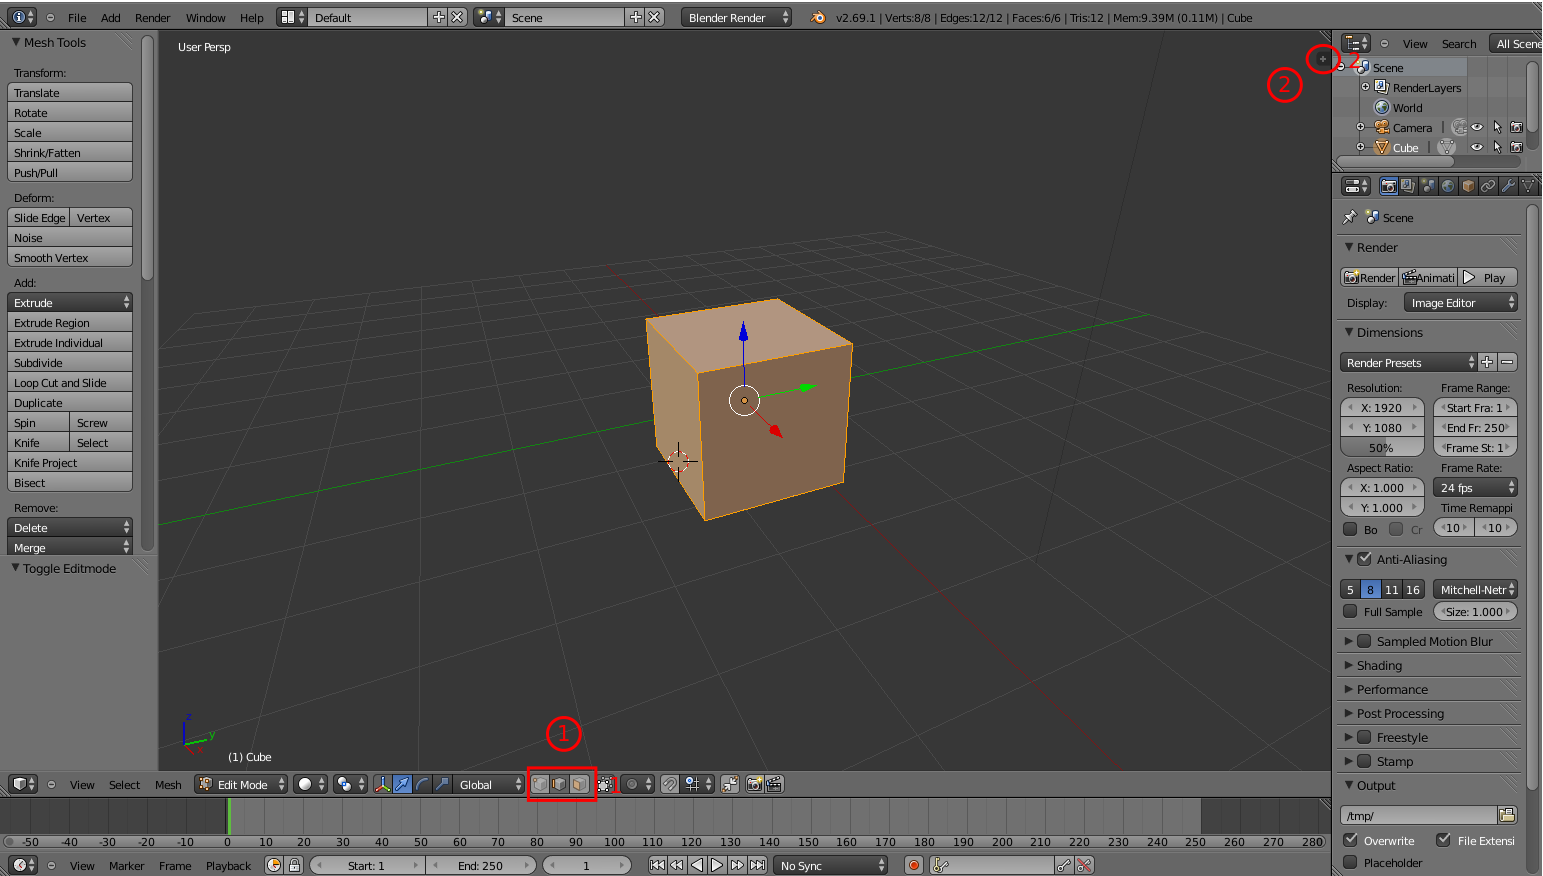
\includegraphics[trim=0cm 0cm 0cm 0cm,clip=true,scale=.17]{Blender_006.png}
	\caption{Blender im \emph{Edit Mode}}
	\label{fig:blender_edit_mode}
	\end{figure}
	\item Im in Abbildung \ref{fig:blender_edit_mode} mit \textbf{1} markierten Bereich der können Sie einstellen, was für eine Art von Elementen Sie bearbeiten wollen. Zur Auswahl stehen \emph{Punkte, Kanten und Flächen}.
	\item Klicken Sie nun mit der \textbf{[rechten Maustaste]} auf das Element, das Sie auswählen möchten. Um mehrere Elemente hintereinander auszuwählen, halten Sie \textbf{[Shift]} gedrückt.
	\item Ausgewählte Elemente können nun verändert werden. Die drei Haupttransformationen sind:
	\begin{itemize}
		\item Verschieben \textbf{[g]}
		\item Rotieren \textbf{[r]}
		\item Skalieren \textbf{[s]}
	\end{itemize}
	Wenn sie die Tasten \textbf{[x],[y] oder [z]} drücken, findet die Transformation nur auf der angegebenen Achse statt. Um welchen Wert Sie das Objekt transformieren wollen, können Sie durch Eingabe von Zahlen (Punkt ist Komma) festlegen. Zum Übernehmen der Änderungen drücken Sie die \textbf{[linke Maustaste]}, zum abbrechen die \textbf{[rechten Maustaste]}.
	\item Klicken Sie auf das auf Abbildung \ref{fig:blender_edit_mode} mit \textbf{2} markierte Kreuz, um eine Seitenleiste zu öffnen, in der Sie die Koordinaten des ausgewählten Elements oder den Median der Koordinaten mehrerer Ausgewählter Elemente einsehen und verändern können.
	\end{itemize}
	\begin{figure}
	\begin{minipage}[h]{.5\textwidth}
		\begin{subfigure}[a]{\textwidth}
			\centering
    			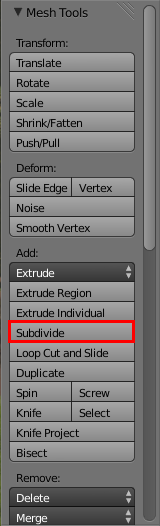
\includegraphics[width=.5\textwidth]{blender_house_subdiv.png}
    			\caption{(b) Unterteilen der Kanten}
    		\end{subfigure}
    \end{minipage}
    \begin{minipage}[h]{.5\textwidth}
		\begin{subfigure}{\textwidth}
			\centering
    			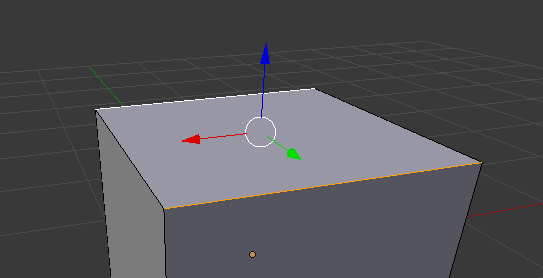
\includegraphics[width=\textwidth]{Blender_house_select.png}
    			\caption{(a) Selektion der Kanten}
    		\end{subfigure}
    
    		\begin{subfigure}[b]{\textwidth}
    			\centering
    			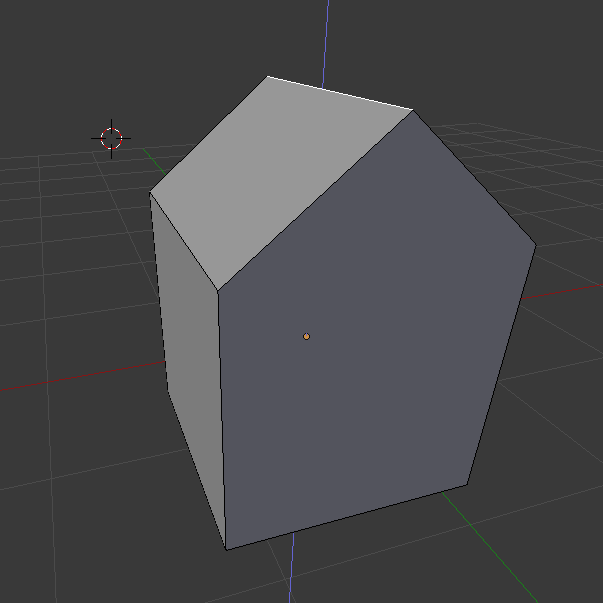
\includegraphics[width=\textwidth]{blender_house.png}
    			\caption{(c) Verschieben der neuen Kante}
    		\end{subfigure}
    \end{minipage}
    \caption{Erstellung eines einfachen Hauses aus dem Standardwürfel}
    \label{fig:blender_house}
	\end{figure}
	Wie aus dem Standardwürfel beispielsweise ein einfaches Haus modelliert werden kann, sehen Sie in Abbildung \ref{fig:blender_house} beschrieben.
	\begin{itemize}
	\item Wählen Sie zwei der oberen Kanten des Würfels mit \textbf{[Shift]} und \textbf{[rechte Maustaste]} aus. 
	\item Klicken Sie auf den Knopf \textbf{[Subdivide]} (Unterteilen) in der linken Seitenleiste.
	\item Wählen Sie nun die entstandene Kante aus. Drücken Sie \textbf{[g]}, danach \textbf{[z]} und geben Sie anschließend \dq 0.8\dq ein. Die Kante ist nun 0,8 Einheiten nach oben verschoben.
	\end{itemize}
	Falls das Objekt in mehrere Materialien untergliedert ist, müssen Sie die Teile, die aus einem bestimmten Material bestehen als einzelne Objekte modellieren. So fügen Sie ein weiteres Objekt hinzu:
	\begin{itemize}
	\item Wechseln Sie durch drücken von \textbf{[TAB]} wieder in den \emph{Object Mode}.
	\item Drücken Sie nun \textbf{[Shift]} und \textbf{[a]} und navigieren sie in das Untermenu \emph{Mesh}.
	\item Wählen Sie mit Klick auf die \textbf{[linke Maustaste]} ein Grundobjekt aus.
	\item Wählen Sie das gerade hinzugefügte Objekt mit Klick auf die  \textbf{[rechte Maustaste]} aus.
	\item Wechseln Sie durch drücken von \textbf{[TAB]} wieder in den \emph{Edit Mode}.
	\item Modellieren Sie das Teilobjekt wie oben beschrieben.
	\end{itemize}
	
	\begin{figure}
	\centering
	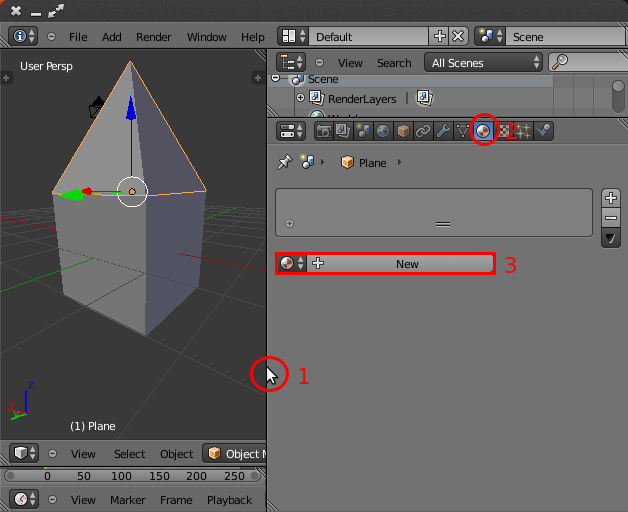
\includegraphics[trim=0cm 0cm 0cm 0cm,clip=true,scale=.4]{blender_newmat.png}
	\caption{Erstellen eines Materials}
	\label{fig:blender_create_mat}
	\end{figure}
	\begin{figure}
	\centering
	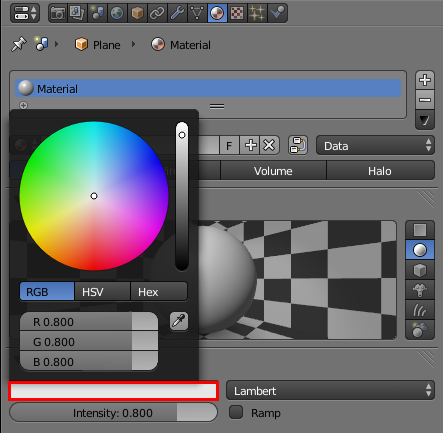
\includegraphics[trim=0cm 0cm 0cm 0cm,clip=true,scale=.34]{blender_mat_col.png}
	\caption{Ändern der Materialfarbe}
	\label{fig:blender_mat_col}
	\end{figure}
	
	Haben Sie alle Teilobjekte erstellt, müssen Sie diesen Materialien zuweisen:
	\begin{itemize}
	\item Wechseln Sie durch drücken von \textbf{[TAB]} wieder in den \emph{Object Mode}.
	\item Wählen Sie mit \textbf{[rechte Maustaste]} ein Teilobjekt aus.
	\item Wechseln Sie zum Reiter \dq Material\dq in den Objekteigenschaften. (\textbf{2} in Abbildung \ref{fig:blender_create_mat}) Wenn dieser nicht zu sehen ist, vergrößern Sie das Eigenschaften-Fenster, indem Sie mit \textbf{[linke Maustaste]} auf die mit \textbf{1} markierte Stelle in Abbildung \ref{fig:blender_create_mat} klicken und die Trennleiste zur Seite ziehen.
	\item Klicken Sie auf \textbf{[New]} (\textbf{3} in Abbildung \ref{fig:blender_create_mat}) und geben Sie einen Namen für das Material ein.
	\item Ändern Sie bei bedarf die Farbe des Materials, indem Sie auf das in Abbildung \ref{fig:blender_mat_col} markierte Feld klicken.
	\end{itemize}
	\begin{warnung}
	Jedes Teilobjekt muss genau ein Material besitzen, auch wenn das Objekt aus nur einem Teilobjekt besteht!
	\end{warnung}
	\begin{figure}
	\centering
	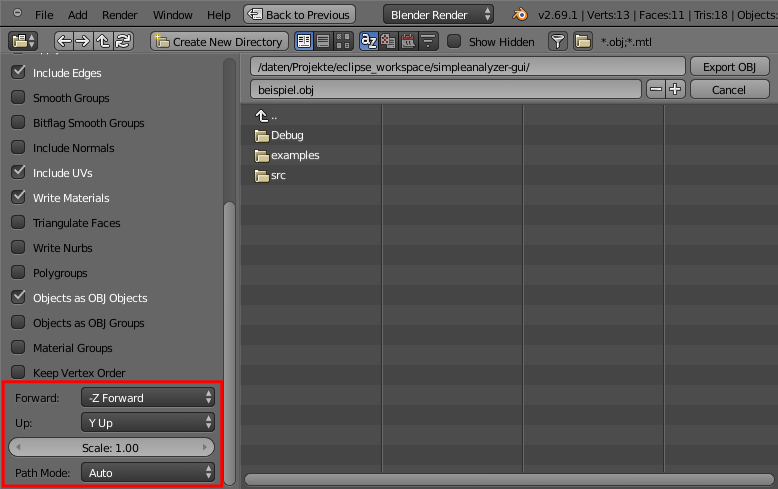
\includegraphics[trim=0cm 0cm 0cm 0cm,clip=true,scale=.33]{blender_export_dlog.png}
	\caption{Exportieren des Objekts}
	\label{fig:blender_export_dlog}
	\end{figure}
	
	Nun kann das Objekt Exportiert werden:
	\begin{itemize}
	\item Navigieren Sie zu \textbf{Datei - Export - Wavefront (.obj)}.
	\item Wählen Sie im in Abbildung \ref{fig:blender_export_dlog} abgebildeten Dialog einen Speicherort für die Datei.
	\item Sollten Achsen des Objekts in \emph{simpleanalyzer-gui} 	vertauscht sein, ändern Sie die in Abbildung \ref{fig:blender_export_dlog} markierten Einstellungen \emph{Forward} und \emph{Up}.
	\end{itemize}
	\newpage
	\subsection{Auswertung und Visualisierung}
	\label{subsec:usage_gui}
	Um die mithilfe der vorher beschriebenen Programme umgewandelten Daten auszuwerten und zu visualisieren, verwenden Sie das Programm \emph{simpleanalyzer-gui}.
	Sie können das Programm entweder über ein Terminal mithilfe des Befehls
	\begin{lstlisting}
	simpleanalyzer-gui
	\end{lstlisting}
	starten, oder indem Sie die Anwendungsverwaltung der Distribution verwenden.
	\begin{hinweis}
	Wenn Sie das Hauptmenü von Programmen in Ubuntu statt am oberen Bildschirmrand direkt unter der oberen Fensterleiste angezeigt haben möchten, deinstallieren Sie das Paket \emph{indicator-appmenu} und melden Sie sich neu an.
	\end{hinweis}
	\subsubsection{Laden von Modellen und Sensordaten}
	\label{subsec:toolbar_and_loading}
	\begin{figure}
	\centering
	
\includegraphics[trim=0cm 0cm 0cm 0cm,clip=true,scale=.5]{Simple_Analyzer_toolbar.png}
	\caption{Die Toolbar}
	\label{fig:sa_toolbar}
	\end{figure}
	Um das Programm sinnvoll einsetzen zu können, benötigen Sie ein 3D-Modell des zu untersuchenden Objekts (s. \ref{subsec:usage_model}) und Sensordaten. Es werden zwei Arten von Sensordatendateien unterstützt:
	\begin{itemize}
	\item Einfache Sensordaten (.sd) enthalten die Koordinaten von Sensoren und ihren Wert zu einem Zeitpunkt.
	\item Zeit-bezogene Sensordaten (.tsd) enthalten die Koordinaten und Werte der Sensoren zu verschiedenen Zeitpunkten. Diese Zeitpunkte können mit eigenen Namen versehen sein.
	\end{itemize}
	Nachdem Sie das Programm gestartet haben, finden Sie im linken Oberen Bereich des Fensters eine Toolbar. Diese bietet Schnellzugriff auf verschiedene Funktionen:
	\begin{itemize}
	\item \textbf{Das 3D-Modell und erste Sensordaten laden:} \\
	Klicken Sie auf das in Abbildung \ref{fig:sa_toolbar} mit \textbf{1} markierte Symbol oder wählen Sie \textbf{Datei - Import - Modell und Sensordaten}. Daraufhin öffnet sich ein Dialog, in dem Sie eine .obj-Datei auswählen können. \\\textbf{WICHTIG:} Zusätzlich zur .obj-Datei muss eine .sd- oder .tsd-Datei mit dem selben Namen vor der Dateiendung im selben Verzeichnis wie die .obj-Datei liegen!
	\item \textbf{Einfache Sensordaten importieren:}\\
	Klicken Sie auf das in Abbildung \ref{fig:sa_toolbar} mit \textbf{2} markierte Symbol oder wählen Sie \textbf{Datei - Import - Sensordaten}. Im sich öffnenden Dialog können Sie eine .sd-Datei auswählen und laden.
	\item \textbf{Zeit-bezogene Sensordaten importieren:}\\
	Klicken Sie auf das in Abbildung \ref{fig:sa_toolbar} mit \textbf{3} markierte Symbol oder wählen Sie \textbf{Datei - Import - Sensordaten-Paket}. Im sich öffnenden Dialog können Sie eine .tsd-Datei auswählen und laden.
	\end{itemize}
	Nachdem Sie ein 3D-Modell und erste Sensordaten geladen haben, berechnet das Programm automatisch eine Temperaturverteilung mit Standardeinstellungen. Sie sehen im in Abbildung \ref{fig:sa_toolbar} mit \textbf{4} markierten Feld den Namen des Objekts, auf das sich alle späteren Operationen beziehen. Wenn Sie mehrere Objekte gleichzeitig untersuchen, können Sie \textbf{zwischen den Objekten umschalten}, indem Sie auf dieses Feld klicken. Nun öffnet sich ein Menü, in dem Sie das Objekt auswählen, mit dem Sie arbeiten möchten.\\
	\begin{hinweis}
	Die Sensordaten sind mit dem Objekt verknüpft, das aktiv war, als diese geladen wurden. Wollen Sie also Sensordaten mit mehreren Objekten nutzen, müssen Sie diese für die betreffenden Objekte jeweils einzeln laden.
	\end{hinweis}
	Wollen Sie ein Objekt wieder löschen, klicken Sie auf das in Abbildung \ref{fig:sa_toolbar} mit \textbf{5} markierte Symbol, um das aktive Objekt zu entfernen. Alternativ kann ein Objekt auch über das Menü unter \textbf{Bearbeiten - Aktives Objekt löschen} entfernt werden.  Wenn das Objekt das einzige geladene Objekt ist, können Sie es nicht löschen!\\
	Durch klicken auf die Symbole \textbf{6} bis \textbf{8} gelangen Sie zu verschiedenen Analysewerkzeugen:
	\begin{itemize}
	\item \textbf{6:} Die Analysedatenübersicht. Siehe \ref{subsec:data_overview}.
	\item \textbf{7:} Die Analyse für einen Punkt. Siehe \ref{subsec:analyze_point}.
	\item \textbf{8:} Die Temperaturverteilung für eine Ebene brerechnen. Siehe \ref{subsec:render_cut}.
	\end{itemize}
	\subsubsection{Berechnen der Temperaturverteilung}
	\label{subsec:temp_vert}
	\begin{figure}
	\centering
	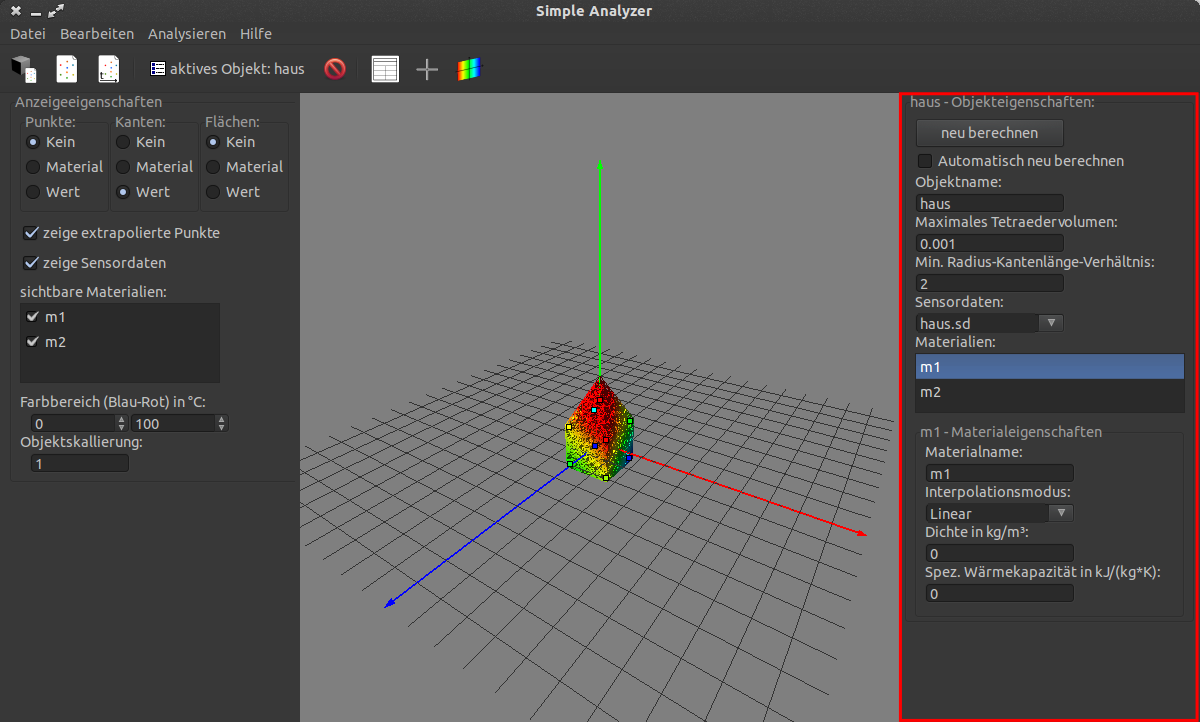
\includegraphics[trim=0cm 0cm 0cm 0cm,clip=true,scale=.2]{Simple_Analyzer_objprops.png}
	\caption{Das Hauptfenster von SimpleAnalyzer}
	\label{fig:sa_objprops}
	\end{figure}
	Nachdem Sie ein Objekt geladen haben, wird automatisch eine Temperaturverteilung mit Standardeinstellungen berechnet. Dabei wird das Objekt in Tetraeder zerlegt, für deren Eckpunkte anschließend eine Temperatur errechnet wird. Um diese erneut mit veränderten Einstellungen zu berechnen, verwenden Sie die in Abbildung \ref{fig:sa_objprops} markierte Seitenleiste:
	\begin{itemize}
	\item \textbf{[neu berechnen]:} Klicken Sie hier, um die Temperaturverteilung neu zu berechnen.
	\item \textbf{Automatisch neu berechnen:} Die Temperaturverteilung automatisch nach jeder Änderung an den Einstellungen automatisch neu berechnen.
	\item \textbf{Objektname:} Der Name des aktuellen Objekts.
	\item \textbf{Maximales Tetraedervolumen:} Maximales Volumen, dass ein Tetraeder bei der Zerlegung haben darf.
	\item \textbf{Min. Radius-Kantenlänge-Verhältnis:} Minimales Verhältnis $\frac{Umkreisradius}{k\ddot{u}rzeste Kantenl\ddot{a}nge}$.
	\item \textbf{Sensordaten:} Wählen Sie hier die zu verwendenden Sensordaten aus. Wenn Sie Zeit-bezogene Sensordaten auswählen, wird eine Zeitleiste eingeblendet. (s. Abbildung \ref{fig:sa_timeline})
	\begin{figure}
	\centering
	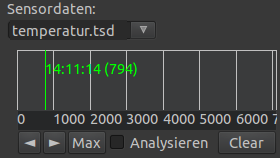
\includegraphics[trim=0cm 0cm 0cm 0cm,clip=true,scale=.54]{Simple_Analyzer_timeline.png}
	\caption{Zeitleiste für eines .tsd-Datensatzes}
	\label{fig:sa_timeline}
	\end{figure}
	Mit der \textbf{[linken Maustaste]} oder mit den \textbf{Pfeiltasten} können Sie den Zeitpunkt auswählen, für den die Temperaturverteilung berechnet werden soll. Der aktuelle Zeitpunkt wird mit Name und Index als grüner Balken angezeigt.\\
	Des Weiteren können Sie den Ausschnitt der Zeitleiste anpassen:
	Verwenden Sie das \textbf{[Mausrad]} um den hinein und hinaus zu zoomen und halten Sie die \textbf{[mittlere Maustaste]} und bewegen Sie die Maus, um den Ausschnitt zu verschieben.\\
	Um für die Auswertung relevante Zeitpunkte zu markieren, aktivieren Sie \textbf{[Analysieren]}. An dieser Stelle wird dadurch eine Markierung gesetzt. Die markierten Zeitpunkte werden in der Analysedatenübersicht (\ref{subsec:data_overview}) angezeigt.
	\begin{itemize}
	\item Klicken Sie die Buttons \textbf{[$<$]} bzw. \textbf{[$>$]} um in die jeweilige Richtung zu einer markierten Stelle zu springen.
	\item Klicken Sie auf \textbf{[Max]}, um den Zeitpunkt, zu dem das Objekt die größte Wärmeenergie enthält, zwischen zwei markierten Stellen zu berechnen. Dazu haben Sie die Wahl zwischen zwei Verfahren: Entweder wird die Temperaturverteilung für jeden Zeitpunkt zwischen den markierten Stellen neu berechnet, oder es wird nur der Durchschnitt der Messwerte verglichen (schneller).
	\item Mit \textbf{[Clear]} können Sie alle Markierungen aufheben.
	\end{itemize}
	\item Klicken Sie auf ein Material unter \textbf{Materialien}, um dessen Eigenschaften im Bereich \textbf{Materialeigenschaften} verändern zu können:
	\begin{itemize}
	\item \textbf{Materialname:} Hier können Sie einen neuen Namen für das Material angeben.
	\item \textbf{Interpolationsmodus:} Wählen Sie hier den Interpolationsmodus für das Material aus.
	\item \textbf{Dichte:} Geben Sie hier die Dichte des Materials in $\frac{kg}{m^3}$ ein.
	\item \textbf{Spez. Wärmekapazität:} Geben Sie hier die spezifische Wärmekapazität der Materials in $\frac{kJ}{kg*K}$ ein.
	\end{itemize}
	\end{itemize}
	\begin{hinweis}
	Wenn eine große Anzahl an Messpunkten vorliegt, kann das Extrapolieren sehr lange dauern. Dies können Sie durch zusätzliche Messpunkte vermeiden. Dies gilt auch für die Analyse des Modells (s. \ref{subsec:sa_analyze}).
	\end{hinweis}
	\subsubsection{Das Modell betrachten}
	\label{subsec:sa_viewprops}
	\begin{figure}
	\centering
	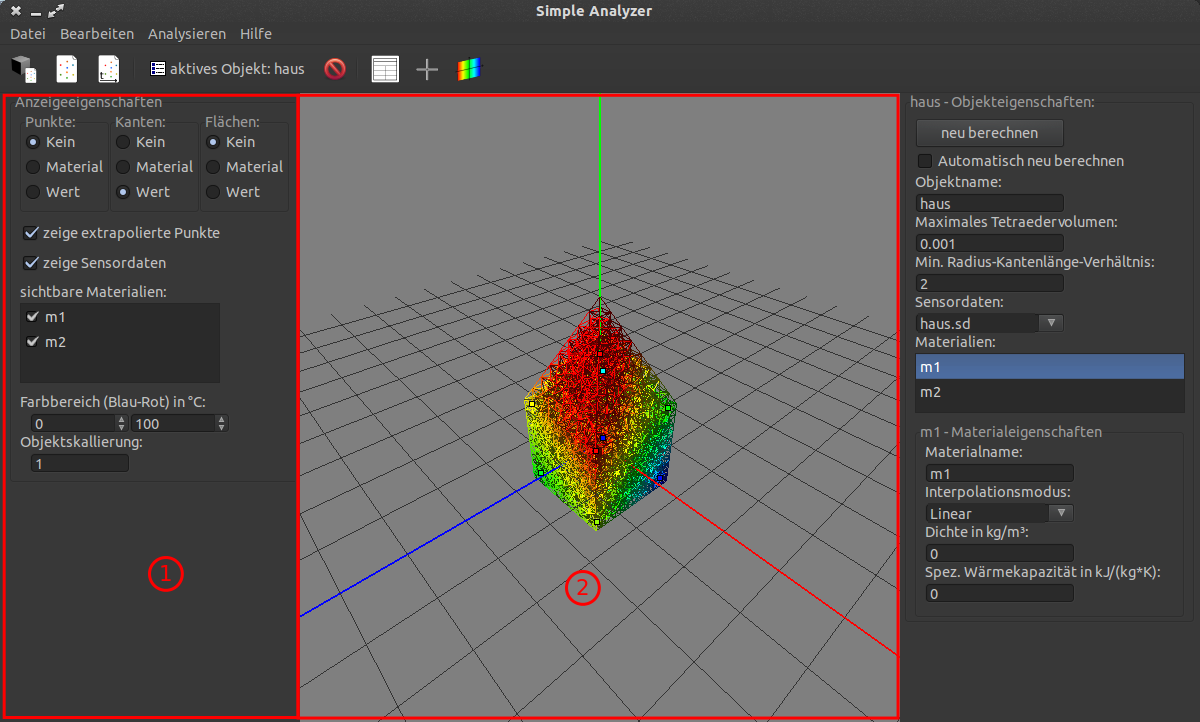
\includegraphics[trim=0cm 0cm 0cm 0cm,clip=true,scale=.2]{Simple_Analyzer_viewprops.png}
	\caption{Das Hauptfenster von SimpleAnalyzer}
	\label{fig:sa_viewprops}
	\end{figure}
	In Abbildung \ref{fig:sa_viewprops} sehen Sie das Hauptfenster von \emph{Sim"-ple"-Ana"-ly"-zer-GUI}. In der Mitte sehen Sie das \textbf{3D-Fenster} (mit \textbf{2} markiert), in dem das aktive Objekt dargestellt wird. Zusätzlich sehen Sie die Achsen des kartesischen Koordinatensystems:\\
	
	\begin{tabular}{ll}
	Rote Linie: & X-Achse\\
	Grüne Linie: & Y-Achse\\
	Blaue Linie: & Z-Achse\\
	\end{tabular}\\
	
	Die Betrachtungsperspektive können Sie wie folgt ändern:
	\begin{itemize}
	\item \textbf{Ansicht drehen:} Halten Sie die \textbf{[linke Maustaste]} über dem 3D-Fenster gedrückt und bewegen Sie die Maus.
	\item \textbf{herein/heraus zoomen:} Scrollen Sie mit dem \textbf{[Mausrad]} vorwärts bzw. rückwärts.
 	\item \textbf{Ansicht verschieben:} Halten Sie die \textbf{[mittlere Maus"=taste]} gedrückt und bewegen Sie die Maus.
	\end{itemize}
	Einstellungen zur Art und Weise, wie das Objekt dargestellt werden soll, können Sie im in Abbildung \ref{fig:sa_viewprops} mit \textbf{1} markieren Bereich verändern:
	\begin{itemize}
	\item \textbf{Punkte/Kanten/Flächen:} Hier können Sie auswählen, ob und wie Punkte im Objekt sowie dessen Kanten und Flächen dargestellt werden. Dabei bedeutet:
	\begin{itemize}
	\item \textbf{Kein:} Diese Art von Elementen (Punkte/Kanten/Flächen) wird nicht angezeigt.
	\item \textbf{Material:} Diese Art von Elementen wird in der Farbe des Materials angezeigt.
	\item \textbf{Material:} Diese Art von Elementen wird der Temperatur entsprechend eingefärbt.
	\end{itemize}
	\item \textbf{zeige extrapolierte Punkte:} Es werden auch Elemente angezeigt, deren Temperatur aus den Messwerten Interpoliert werden musste.
	\item \textbf{zeige Sensordaten:} Die Sensordaten werden als große farbige Punkte mit im Modell angezeigt.
	\item \textbf{sichtbare Materialien:} Es werden nur die Elemente angezeigt, die zu einem der mit einem Haken versehenen Materialien gehören. Möchten Sie ein Material ausblenden, entfernen Sie den Haken vor dem entsprechenden Material.
	\item \textbf{Farbbereich:} Die Temperatur im linken Feld entspricht in der Visualisierung der Farbe Blau (geringste Temperatur), die im rechten Feld der Farbe rot (höchste Temperatur). Durch verändern dieser Werte können Sie beeinflussen, wie die Temperatur eines Elements farblich dargestellt wird.
	\item \textbf{Objektskalierung:} Das Objekt um diesen Faktor vergrößert darstellen. Die Skalierung ist dabei rein optisch.
	\end{itemize}
	\newpage
	\subsection{Analyse des Modells}
	\label{subsec:sa_analyze}
	Das Programm auch Möglichkeiten zur Analyse der berechneten Temperaturverteilung. 
	\subsubsection{Die Analysedatenübersicht}
	\label{subsec:data_overview}
	\begin{figure}
	\centering
	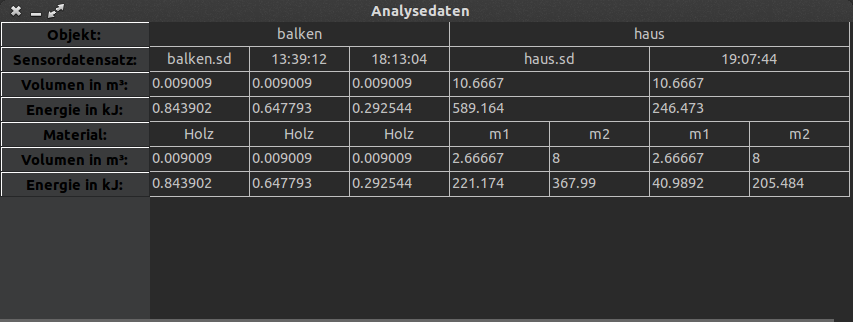
\includegraphics[trim=0cm 0cm 0cm 0cm,clip=true,scale=.3]{SA_overview.png}
	\caption{Das Übersichtsfenster}
	\label{fig:sa_data_overview}
	\end{figure}
	Navigieren Sie im Hauptmenü zu \textbf{Analysieren - Übersicht} oder wählen Sie das entsprechende Symbol auf der Toolbar (s. \ref{subsec:toolbar_and_loading}), um eine Übersicht über den \textbf{Wärmeenergiegehalt} aller geladenen Objekte angezeigt zu bekommen. Angezeigt werden der \emph{des Objekts, Energiegehalt der einzelnen Materialien für alle mit diesem Objekt verknüpften Datensätze und das Volumen dieser}.
	Wenn ein Objekt Zeit-bezogene Sensordaten besitzt, müssen Sie die zu analysierenden Zeitpunkte erst markieren(s. \ref{subsec:temp_vert}). 
	\begin{hinweis}
	Um die Analysedaten z.B. in ein Tabellenkalkulationsprogramm zu übernehmen, markieren Sie alle Zellen der Tabelle, indem Sie in diese klicken und anschließend die Tasten \textbf{[Strg]} + \textbf{[a]} drücken. Kopieren Sie nun deren Inhalte mit \textbf{[Strg]} + \textbf{[c]}. Die Werte sind nun in der Zwischenablage ihres Systems gespeichert und können in andere Programme wieder eingefügt werden.
	\end{hinweis}
	\begin{hinweis}
	Solange Sie das Übersichtsfenster geöffnet haben, wird das Fenster automatisch aktualisiert, sobald Sie ein Objekt neu berechnen.
	\end{hinweis}
	\begin{hinweis}
	Für die Berechnung des Energiegehalts ist es wichtig, dass Sie für alle Materialien eine spezifische Wärmekapazität und eine Dichte festgelegt haben! (s. \ref{subsec:temp_vert})
	\end{hinweis}
	\subsubsection{Analyse für einen Punkt}
	\label{subsec:analyze_point}
	\begin{figure}
	\centering
	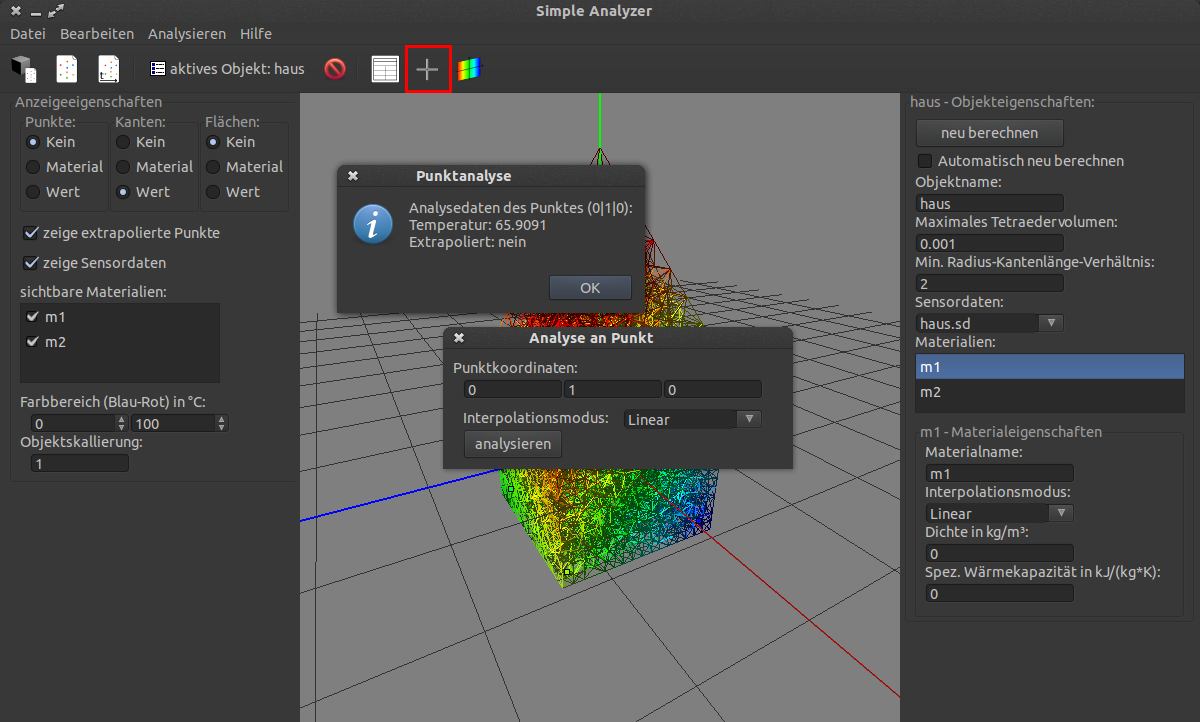
\includegraphics[trim=0cm 0cm 0cm 0cm,clip=true,scale=.2]{SA_analyze_point.png}
	\caption{Analyse an einem Punkt}
	\label{fig:sa_analyze_point}
	\end{figure}
	Um Informationen über einen einzelnen Punkt im Modell zu erhalten, wählen Sie das in Abbildung \ref{fig:sa_analyze_point} markierte Symbol in der Toolbar oder den Menüpunkt \textbf{Analysieren - Punkt}. Es öffnet sich ein Fenster, in dem Sie die Koordinaten des Punktes und den Interpolationsmodus festlegen können. Klicken Sie auf \textbf{[analysieren]}, um die Temperatur des Punktes in $^{\circ}\mathrm{C}$ anzuzeigen. Zusätzlich zeigt die Meldung, ob der Punkt inter- oder extrapoliert wurde. 
	\begin{hinweis}
	\dq extrapoliert\dq \space bedeutet nicht das er sich außerhalb des Objekts befindet, sondern dass der Punkt außerhalb des durch die Messpunkte umgebenen Volumens ist.
	\end{hinweis}
	\subsection{Temperaturverteilung einer Ebene}
	\label{subsec:render_cut}
	\begin{figure}
	\centering
	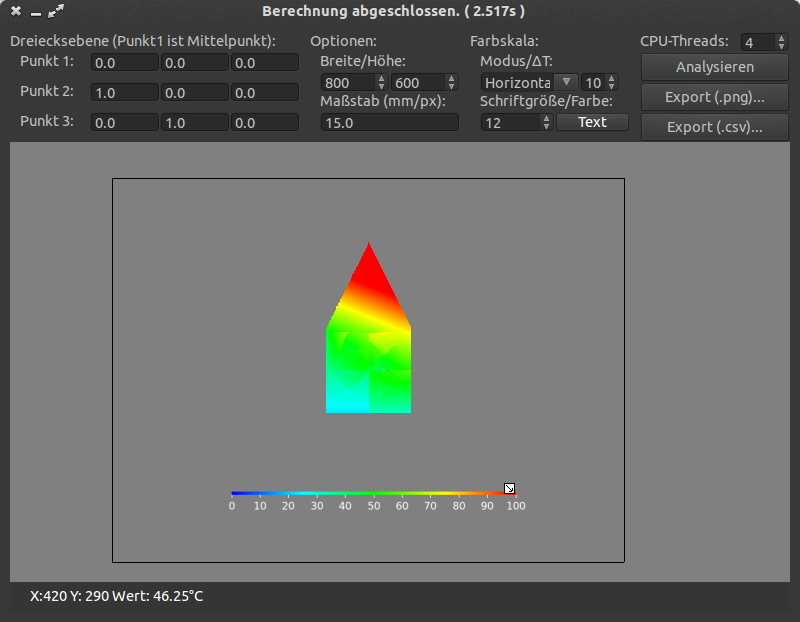
\includegraphics[trim=0cm 0cm 0cm 0cm,clip=true,scale=.3
	]{SA_render_cut.png}
	\caption{Fenster zur 2D-Temperaturverteilung}
	\label{fig:sa_render_cut}
	\end{figure}	
	Um die Temperaturverteilung einer Ebene (als Grafik) zu berechnen, wählen Sie im Menü \textbf{Analysieren - Schnitt berechnen} oder klicken Sie auf das entsprechende Symbol auf der Toolbar (s. \ref{subsec:toolbar_and_loading}). Sie sehen nun das Fenster zur Berechnung einer Schnittebene durch das Objekt. Diese Ebene wird im 3D-Fenster des Hauptfensters mithilfe eines roten und grünen Pfeils angezeigt. Der rote Pfeil stellt dabei die X-Achse, der Grüne die Y-Achse der Ebene dar. An ihrem Schnittpunkt befindet sich die Mitte der Ebene, der später dargestellte Ausschnitt wird durch ein schwarzes Rechteck dargestellt. Zusätzlich wird das Dreieck, das die Ebene definiert, halb-transparent eingezeichnet (s. Abbildung \ref{fig:sa_vis_cut}).
	\begin{figure}
	\centering
	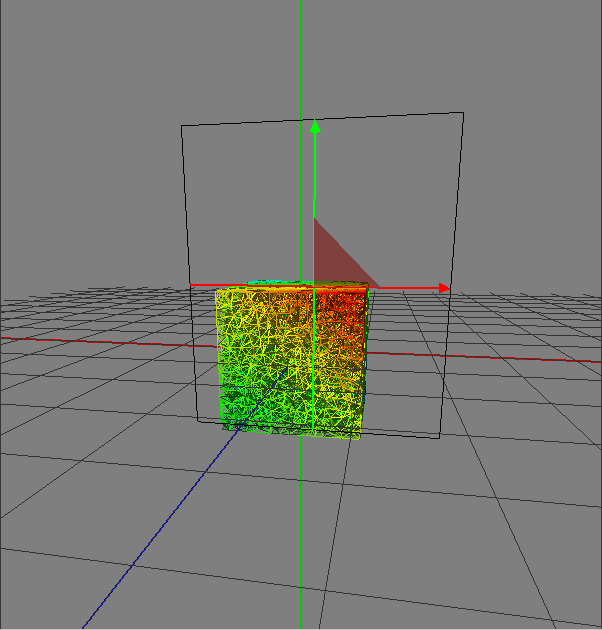
\includegraphics[trim=0cm 0cm 0cm 0cm,clip=true,scale=.3
	]{render_cut_vis.png}
	\caption{Visualisierung im Hauptfenster}
	\label{fig:sa_vis_cut}
	\end{figure}	
	Die Eigenschaften der Ebene und der resultierenden Grafik können Sie im Fenster zur Schnittberechnung einstellen:
	\begin{itemize}
	\item \textbf{Dreiecksebene:} Legen Sie hier die Eckpunkte des Dreiecks fest, das die Ebene beschreibt. Dabei ist der erste Punkt die Mitte des untersuchten Bereichs. \textbf{Die Lage der Ebene wird im Hauptfenster visualisiert.}
	\item \textbf{Optionen:} Hier finden Sie weitere Einstellungen zur resultierenden Grafik:
	\begin{itemize}
	\item \textbf{Breite/Höhe:} Die Maße der Grafik.
	\item \textbf{Maßstab (mm/px):} Der Maßstab der Grafik zum Objekt in $\frac{mm}{Pixel}$. 
	\end{itemize}
	\item \textbf{Temperaturskala:} 
	Hier finden Sie Einstellungen bezüglich der Temperaturskala der Grafik. 
	\begin{itemize}
	\item \textbf{Modus/$\Delta T$}: Ausrichtungsmodus der Temperatur"=skala (\emph{horizontal, vertikal, keine}) und Schrittweite der Beschriftung in $K$.
	\item \textbf{Schriftgröße/Farbe}: Schriftgröße und Schriftfarbe.  Klicken Sie auf \textbf{[Text]}, um einen Dialog zur Auswahl der Schriftfarbe zu öffnen.
	\end{itemize}
	Um die \textbf{Position} der Temperaturskala zu ändern, klicken Sie auf eine Farbige stelle der Skala, halten sie die \textbf{[linke Maustaste]} gedrückt und ziehen Sie sie an den gewünschten Ort.\\
	Zum ändern der \textbf{Größe} klicken Sie auf das weiße Rechteck mit schwarzem Rahmen und Pfeil an der unteren rechten Ecke der Skala und ziehen Sie die diese mit gedrückter \textbf{[linker Maustaste]} in die gewünschte Größe.
	\item \textbf{CPU-Threads:} Geben Sie hier die Anzahl der Threads an, die zum berechnen Verwendet werden sollen. Um die kleinste Rechendauer zu erreichen, sollte dieser Wert der Anzahl ihrer Prozessorkerne entsprechen.
	\end{itemize}
	Das berechnete Bild wird nun im unteren Teil des Fensters angezeigt. Durch gedrückt halten der \textbf{[linken Maustaste]} und ziehen mit der Maus können Sie die Ansicht auf das Bild verschieben. Mit dem \textbf{[Mausrad]} können Sie hinein und hinaus zoomen.\\
	In der Statusleiste am unteren Rand des Fensters finden Sie die Position des Mauszeigers auf dem Bild und den entsprechenden Temperaturwert, falls sich der Mauszeiger über dem Objekt befindet.
	\begin{hinweis}
	Für die Einfärbung der Grafik wird der selbe Farbbereich wie auch für das 3D-Fenster verwendet. (s. \ref{subsec:sa_viewprops})
	\end{hinweis}
	Klicken Sie auf \textbf{[Analysieren]}, um die Berechnung der Grafik zu starten. Klicken Sie anschließend auf \textbf{[Export (.png)]}, um diese als Bilddatei zu exportieren. Alternativ können Sie die Grafik als .csv-Tabelle exportieren, indem Sie auf \textbf{[Export (.csv)]} klicken.
	\begin{hinweis}
	Wenn Sie die Datei als .csv-Tabelle exportieren, ist es meist sinnvoll eine geringe Auflösung zu wählen, da jedem Pixel der Grafik eine Zelle in der Tabelle entspricht.
	\end{hinweis}
	\newpage
	\subsection{Exportmöglichkeiten}
	\label{subsec:sa_export}
	Die durch das Programm ermittelten Daten können zur weiteren Verwendung exportiert werden. \textbf{Für die Temperaturverteilung über eine Ebene sind die Exportmöglichkeiten bereits in \ref{subsec:render_cut} beschrieben.}
	\subsubsection{Anzeige des 3D-Fensters}
	\begin{figure}
	\centering
	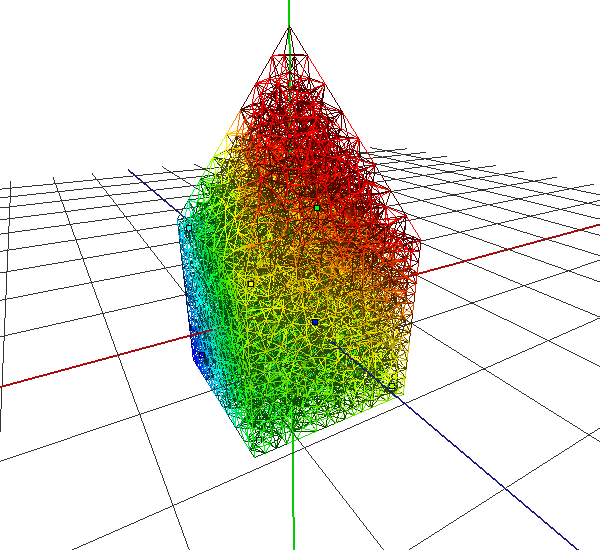
\includegraphics[trim=0cm 0cm 0cm 0cm,clip=true,scale=.3]{SA_export_view.png}
	\caption{Aus dem 3D-Fenster exportiertes Bild}
	\end{figure}	
	Wählen Sie \textbf{Datei - Export - Screenshot (Viewport)}, um das Bild, dass das 3D-Fenster gerade anzeigt, als Bilddatei zu Speichern. Um einen transparenten Hintergrund zu erzeugen, speichern Sie das Bild als .png-Datei.
	\subsubsection{VTK-Datei}
	\begin{figure}
	\centering
	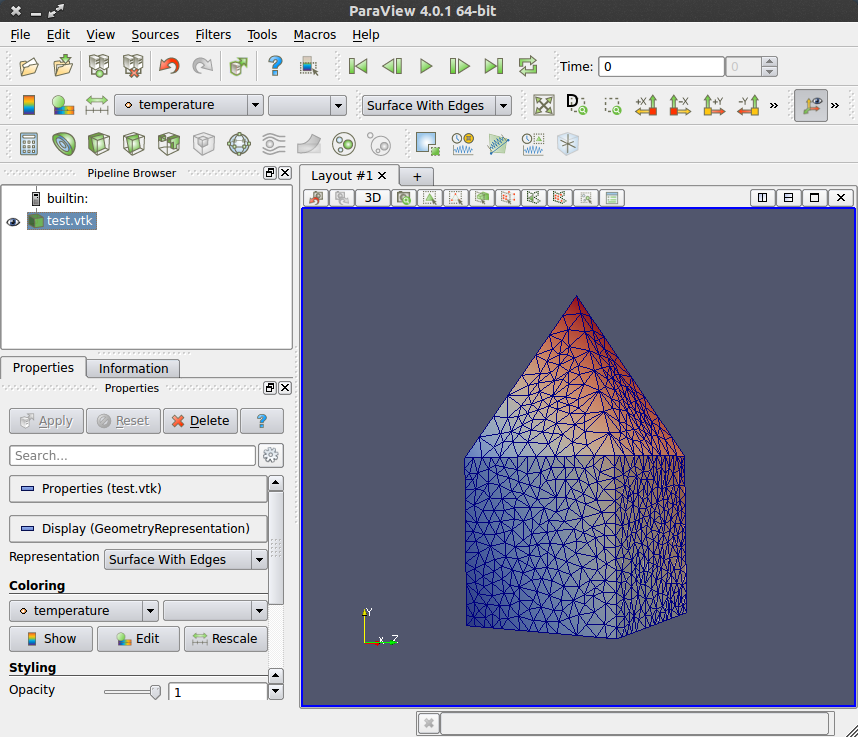
\includegraphics[trim=0cm 0cm 0cm 0cm,clip=true,scale=.3
	]{vtk_paraview.png}
	\caption{Die exportierte VTK-Datei in ParaView}
	\end{figure}	
	Wählen Sie \textbf{Datei - Export - Legacy VTK-Datei}, um das Objekt als Visualisation-Toolkit-Datei zu exportieren. Diese Dateien können in vielen Programmen zur Visualisierung verwendet werden (bspw. \emph{ParaView}).
	\newpage
	\section{Generelles Vorgehen}
	Im Folgenden finden Sie das allgemeine Vorgehen zur Auswertung der meisten Versuche.
	\begin{enumerate}
	\item Wandeln Sie die Messwerte der Punktsensoren aus den .csv-Dateien in .tsd-Dateien um und passen Sie wenn nötig das Format der Eingabedatei an. z.B.:\\
	Inhalt der Sensordefinitions-Datei:
	\begin{lstlisting}
	#name x y z
	"1 - TK_1.1" 0.125 0.035 0.09
	"2 - TK_1.2" 0.125 0.035 0.03
	"5 - TK_1.5" 0.125 0.105 0.09
	"6 - TK_1.6" 0.125 0.105 0.03
	"3 - TK_1.3" 0.375 0.035 0.09
	...
	\end{lstlisting}	
	Befehl zum Umwandeln:
	\begin{lstlisting}
	csvtosd -i input.csv -o points.tsd -s sensors.sdef
	\end{lstlisting}	
	\item Wandeln Sie die ODiSI-Messwerte in .tsd-Dateien um und passen Sie wenn nötig das Format der Eingabedatei an. z.B.:\\
	Inhalt der Sensordefinitions-Datei:
	\begin{lstlisting}
	#odisi definition file
	#type (in/out)    position  x
	i 0.60 .084
	o 0.73 .084
	i 0.83 .167
	o 0.96 .167
	i 1.05 .248
	o 1.18 .248
	...
	\end{lstlisting}	
	Befehl zum Umwandeln:
	\begin{lstlisting}
	odisitosd -i input.txt -o odisi.tsd -s sensors.sdef -l log.txt
	\end{lstlisting}	
	
	\item Führen Sie alle Sensordatensätze zusammen. z.B.:\\
	Befehl zum Zusammenführen:
	\begin{lstlisting}
	mergetsd -i1 points.tsd -i2 odisi.tsd -o versuch.tsd
	\end{lstlisting}	
	Um mehr als zwei Sensordatensätze zusammenzuführen, vereinigen Sie jeweils zwei Dateien zu einer neuen, von denen vereinigen Sie wiederum zwei, bis Sie alle Daten in einer Datei zusammengeführt haben.
	\item Erstellen Sie das 3D-Modell. Dafür können Sie beispielsweise die freie Software \emph{Blender} verwenden, wie bereits in \ref{subsec:3dmodel_blender} beschrieben.
	\item Laden Sie Modell und Sensordaten. Passen Sie anschließend die Objekt- und Materialeigenschaften an. (s. \ref{subsec:usage_gui})
	\item Je nach benötigten Daten können Sie nun:
	\begin{itemize}
	\item die Temperatur an einem Punkt oder Wärmeenergiegehalt des Modells bestimmen. (s. \ref{subsec:sa_analyze})
	\item die Temperaturverteilung über eine Ebene berechnen. (s. \ref{subsec:render_cut})
	\item die Temperaturverteilung oder die Anzeige des 3D-Fensters exportieren. (s. \ref{subsec:sa_export})
	\end{itemize}
	\end{enumerate}
	\label{sec:example}
	
\section{Fehlerbehebung}
\subsection{Bei der Konvertierung}
\begin{tabular}{p{2.cm}|p{6.3cm}}
\textsc{Problem} & \textsc{Lösungsansatz}\\
\hline
\vspace{1em}&\vspace{1em}\\
csvtosd oder odisitosd stürzt ab & Prüfen Sie, ob das Format der jeweiligen Ausgangsdatei oder Sensordefinitionsdatei korrekt ist und mit der Konfigurationsdatei übereinstimmt.\\
& Prüfen Sie, ob alle verwendeten Dateien ASCII-Codiert und mit Linux-Zeilenenden versehen sind. Um dies zu testen, können sie den Befehl

\texttt{file <Datei>}

verwenden. Um eine Datei ggf. entsprechend umzuwandeln, verwenden Sie \textbf{dos2unix} (s. \ref{subsec:csvtosd}).\\
\vspace{1em}&\vspace{1em}\\
csvtosd findet Sensordefinitionen nicht & Prüfen Sie, ob die Sensornamen in Datendatei und Sensordefinitionsdatei einheitlich sind. Wenn Sie Sensornamen mit Leerzeichen verwenden, müssen \textbf{nur} in der Sensordefinitionsdatei in Anführungszeichen gesetzt werden! Prüfen Sie auch die Zeichencodierung der Datei (s. o.).\vspace{1em}\\

mergetsd fügt die Dateien Zeitversetzt zusammen & Verändern Sie die zeitliche Verschiebung der Dateien (-offset). Siehe \ref{subsec:mergetsd}.\\
\end{tabular}

\subsection{Bei der Auswertung}
\begin{tabular}{p{2cm}|p{6.3cm}}
\textsc{Problem} & \textsc{Lösungsansatz}\\
\hline
\vspace{1em}&\vspace{1em}\\
Dichte und spezifische Wärmekapazität des Materials werden nicht übernommen &
Nach jeder Änderung an den Objekteigenschaften muss dieses neu Berechnet werden, um die Änderungen zu speichern. Dies gilt auch, wenn ein anderes Material in den Objekteigenschaften ausgewählt wird und die Eigenschaften des vorher Ausgewählten gespeichert werden sollen.\\
\vspace{1em}&\vspace{1em}\\

Das Objekt ist in der 3D-Ansicht bei hohem Zoom nur Teilweise zu sehen. & Das Objekt kann nur bis zu einer bestimmten nähe der virtuellen Kamera dargestellt werden. Um dennoch Details am Objekt erkennen zu können, können Sie das Objekt in den Visualisierungsoptionen optisch skalieren. (Siehe \ref{subsec:sa_viewprops})
\end{tabular}
\newpage
\section{Lizenzbestimmungen}

SimpleAnalyzer is a simple analyzer for temperature data including converter tools. \\
Copyright (C) 2013-2014 Valentin Roland\\

This program is free software: you can redistribute it and/or
modify it under the terms of the GNU Affero General Public License
as published by the Free Software Foundation, either version 3 of
the License, or (at your option) any later version.\\

This program is distributed in the hope that it will be useful,
but WITHOUT ANY WARRANTY; without even the implied warranty of
MERCHANTABILITY or FITNESS FOR A PARTICULAR PURPOSE.  See the GNU
Affero General Public License for more details.\\

You can find a copy of the GNU Affero General Public License in the LICENSE file provided in the SimpleAnalyzer repository or at \url{http://www.gnu.org/licenses/}.\\

This software makes use of the version 1.5 of the tetgen library, which is licensed under the terms of the GNU Affero General Public License. (see \url{www.tetgen.org})

\end{document}
